\section{Experimental Evaluation} 
\label{sec:Eval} 


This section presents experiments to evaluate how much running time costs in terms of performance. The experiments will show that, in practice, \dyntset is faster by a factor of $O(\log n)$ per operation than that of the theoretical analysis (Section\ref{sec:TechDes}).

This section is organised as follows. Firstly, we describe the experimental setup. Secondly, a brief description in the implementation of test sets is provided. We then present experimental studies of the three different operations in \dyntset. Finally, we present an additional experiment for the cases where laziness as speeding up factor in favor of the running times for the dynamic tree operations.


\subsection{Experimental Setup}
Functions \link, \cut, \conn, \code{root} and \code{reroot} were implemented by the author in Haskell and compiled with \code{ghc} version 8.0.1 with optimisation \code{-O2}. The experiments were performed on a 2.2 GHz Intel Core i7 MacBook Pro with 16 GB 1600 MHz DDR3 running macOS High Sierra version 10.13.1 (17B1003). We imported the following libraries into our code from the online package repository Hackage: \cite{HaskellFT} code for finger trees, \cite{HaskellSet} for conventional sets and \cite{HaskellEdison} for lazy sets.

The running time of a given computation was determined by the mean of three executions.

\subsection{Data structure} 

The values maintained by the data structures (sets and finger trees) are stored as fixed-precision \code{Int} types, holding values from $-2^{29}$ up to $2^{28}$ although we test only the positive values.

The structures are initialized with a fixed number of nodes (or vertices) $n$; this number does not change during the execution. This allow us to know the initial size of the forest and we subtract it from the benchmarking.

Since \dyntset is not called by any application, the random generation of nodes for \link or \cut does not necessarily be effective. Actually, around 70\% of the generated nodes $x$ and $y$ passed to \link and \cut were not valid, that is, their result turned out to be the original forest. In order to overcome this, we stored the random generated nodes that were effective into a plain files and from there benchmarking the dynamic tree operations.


\subsection{Incremental operations} 
We start with an empty forest (just singleton-trees); given $n=20,000$ nodes we perform $1 \ldots 20,000$ \link operations. Upon reaching a target length, we plot the total time taken. Then, we divide the time taken by the number of operations to calculate the time per operation and then multiply it by a constant (x1000) to make the curve visible in the same chart.

\begin{figure}[H]
\begin{center}
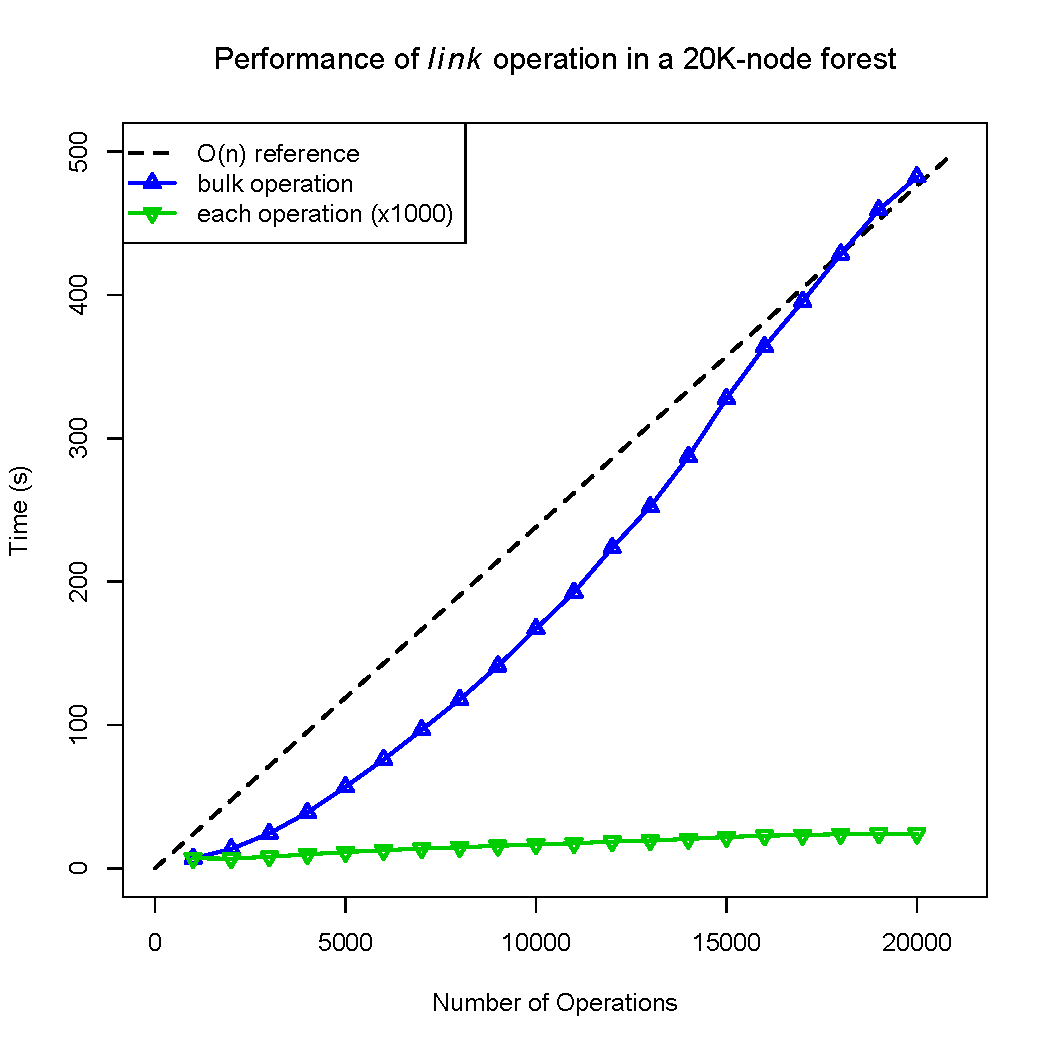
\includegraphics[scale=0.4]{./Images/plotLink} 
\end{center}
\caption{Sequence of {\link}s from empty forest up to a single tree in such forest}
\label{fig:incLink}
\end{figure}

\textit{\emph{Results}}. The behaviour of the curve regarding the time per \link operation shows that in practice it takes $O(1)$ against $O(\log n^2)$ in theory back in Section~\ref{sec:TechDes}, or the linear behaviour by the \link operations in bulk.

\subsection{Fully dynamic operations} 
We start with the incremental process as before for $n=10,000$. Then, for \cut we start in the opposite direction, that is, cutting from a single tree in the forest until only singleton-trees remain in such forest. To this performance we subtract the time take for the incremental bit. For \conn performance we compute first an interleaved operation of \link and \cut (not necessarily in this order). We measure the time taken for \conn followed by the corresponding \link or \cut and then we subtract the interleaved process. The following figures show our three dynamic operations in bulk and per operation.

\begin{figure}[H]
\centering
\begin{subfigure}{.5\textwidth}
  \centering
  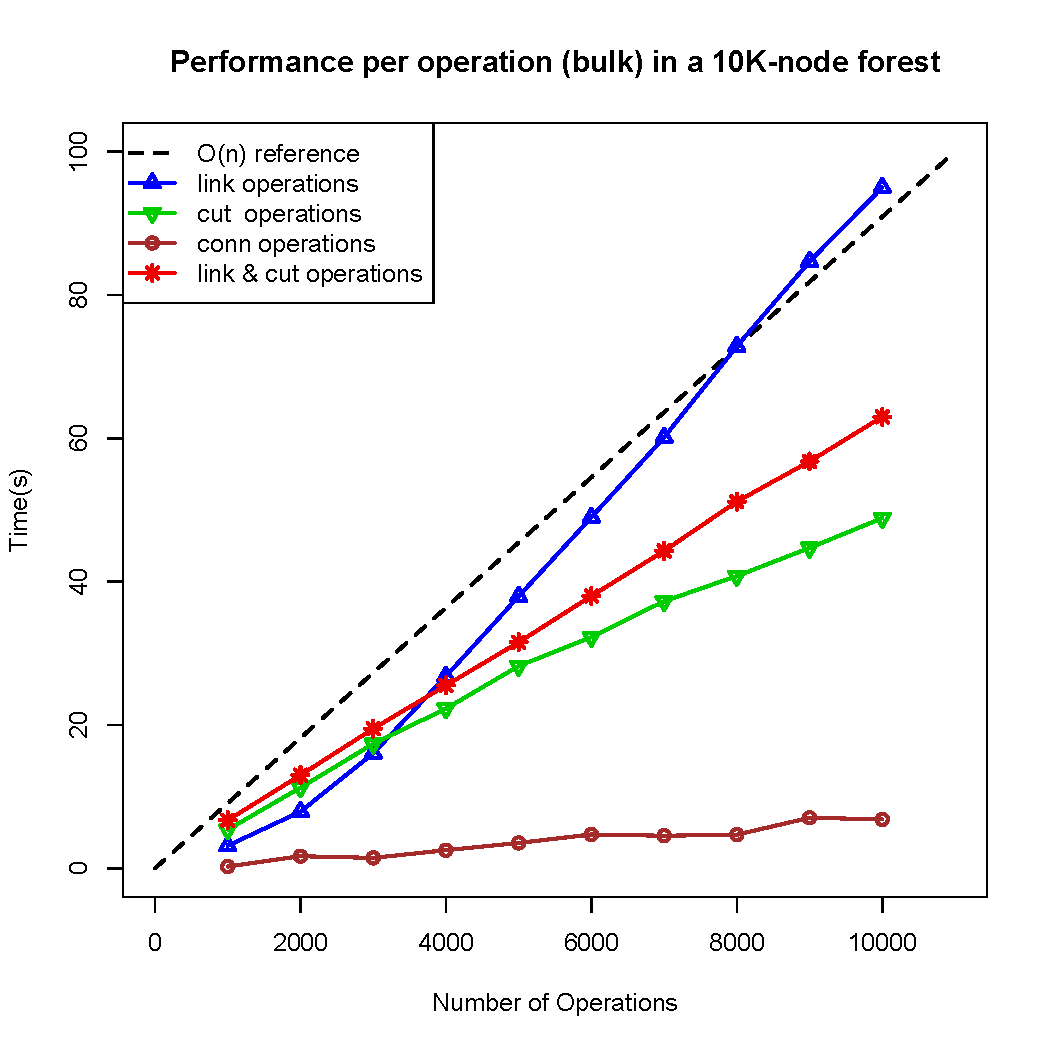
\includegraphics[scale=0.38]{./Images/plotEach}
  \caption{In bulk}
%  \label{fig:sub1}
\end{subfigure}%
\begin{subfigure}{.5\textwidth}
  \centering
  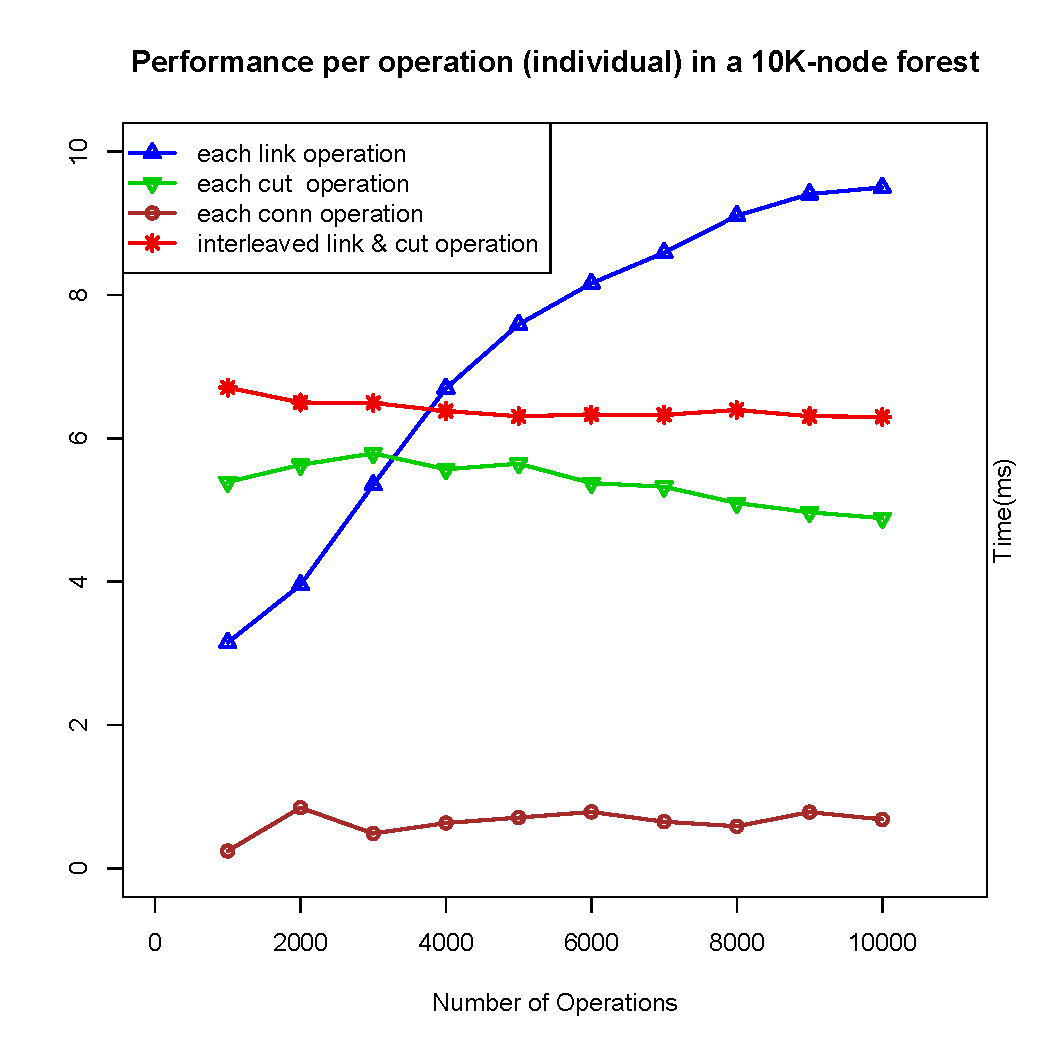
\includegraphics[scale=0.38]{./Images/plotOpsIndiv}
  \caption{Per operation}
%  \label{fig:sub2}
\end{subfigure}
\caption{Time taken by operation, and interleaved \link and \cut}
\label{fig:EachOp}
\end{figure}

\textit{\emph{Results}}. We observe that \cut and \conn obey the same pattern as \link. That is, $O(1)$ time per operation being \textit{connectivity} the fastest of the dynamic tree operations, as expected.

From the above analyses, we notice that \link performs better when is interleaved with \cut. To see this behaviour closer, we present the bulk and individual cases in the following charts varying the forest size under the same amount of operations.

\begin{figure}[H]
\centering
\begin{subfigure}{.5\textwidth}
  \centering
  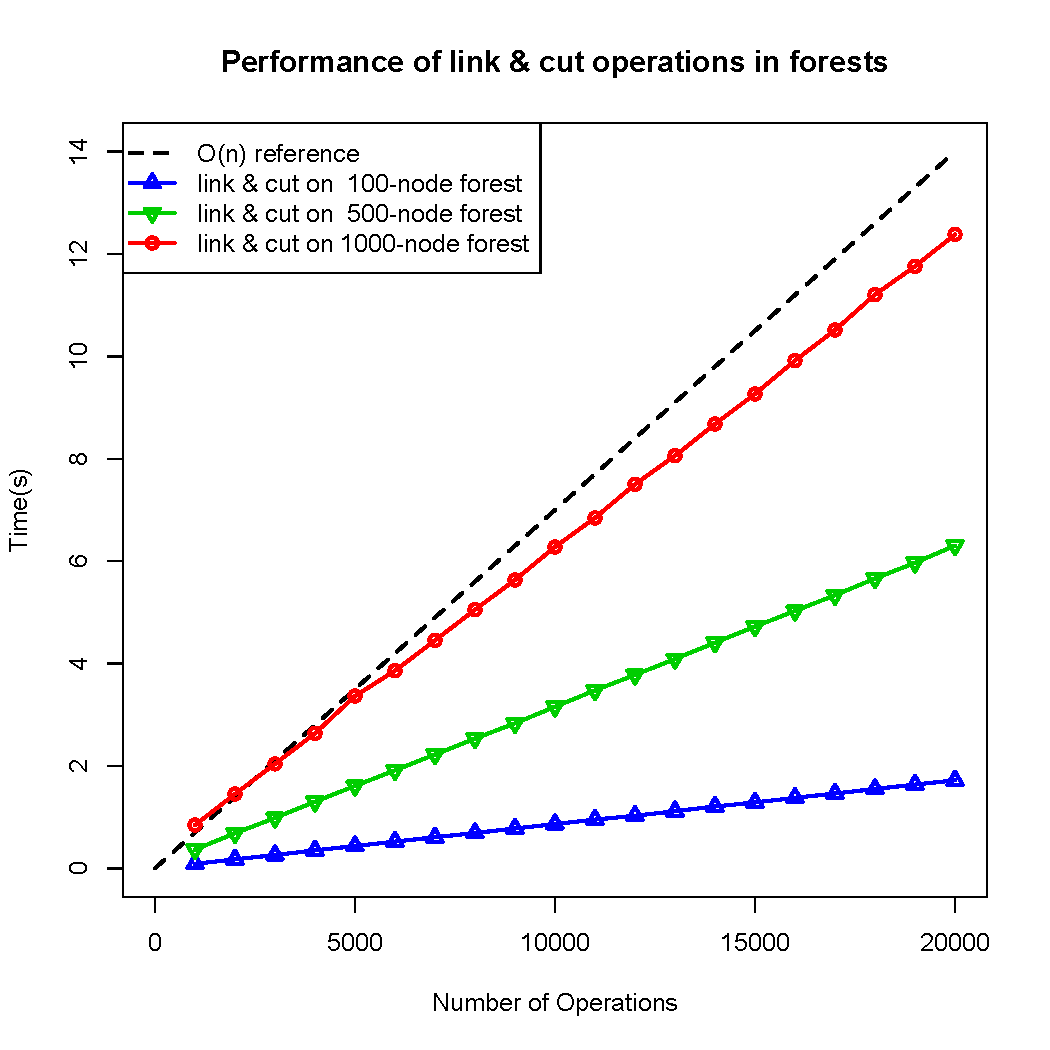
\includegraphics[scale=0.38]{./Images/plotForests}
  \caption{In bulk}
%  \label{fig:sub1}
\end{subfigure}%
\begin{subfigure}{.5\textwidth}
  \centering
  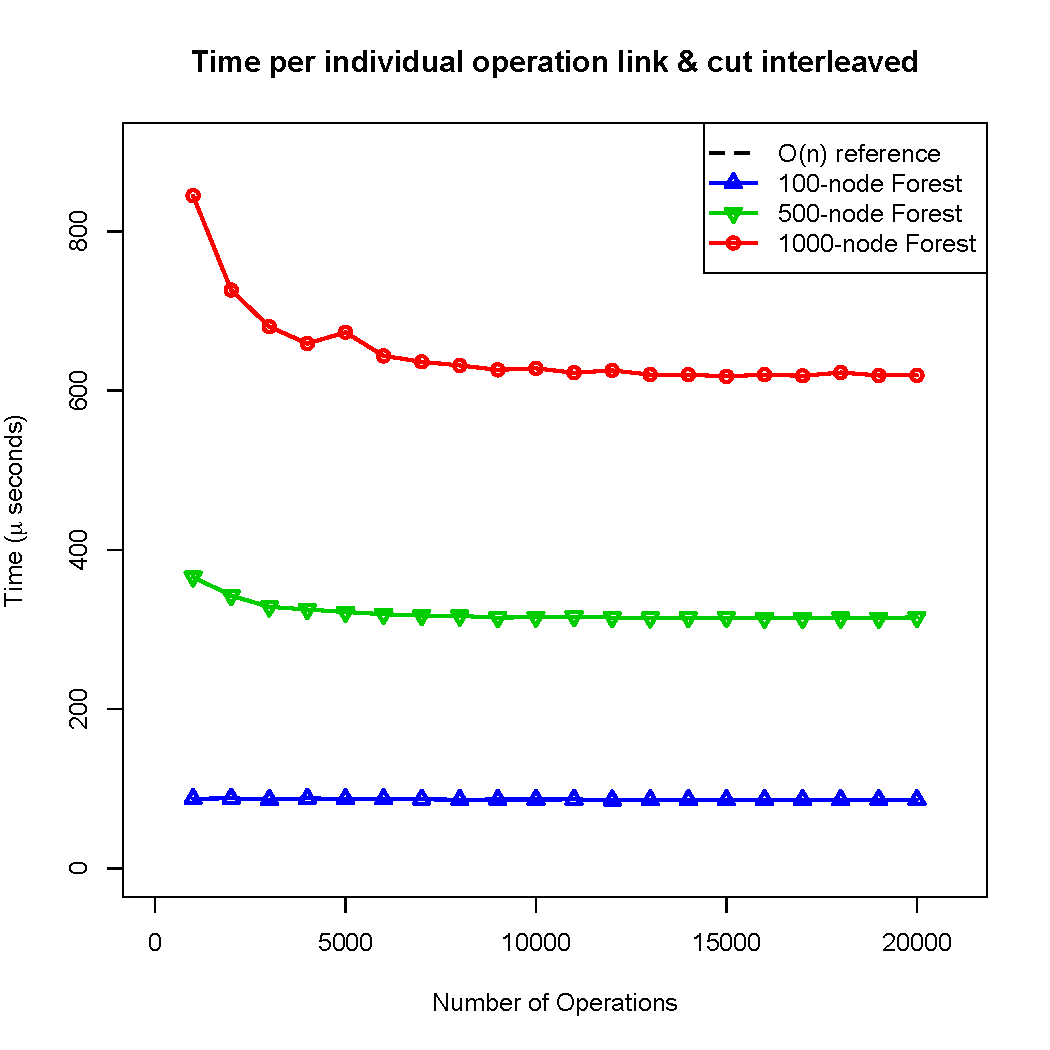
\includegraphics[scale=0.38]{./Images/plotLCForests}
  \caption{Per operation}
%  \label{fig:sub2}
\end{subfigure}
\caption{Time taken when \link and \cut are interleaved with different forest sizes}
\label{fig:EachOp}
\end{figure}

\subsection{Selection of the set data structure}
The set-like data structure is crucial in our implementation and testing of \dyntset since is the search engine for the nodes when any operation is applied to a forest. There are plenty of implementations for such set-like structure, mostly as binary balanced search trees. In our case, where Haskell is a lazy-evaluation language by default, we select two main choices to compare: \code{Data.Set} which is a strict data type definition and \code{Data.Edison.Coll.LazyPairingHeap} which is semi-lazy or semi-strict data type. The following figure shows the performance for each.

\begin{figure}[H]
\begin{center}
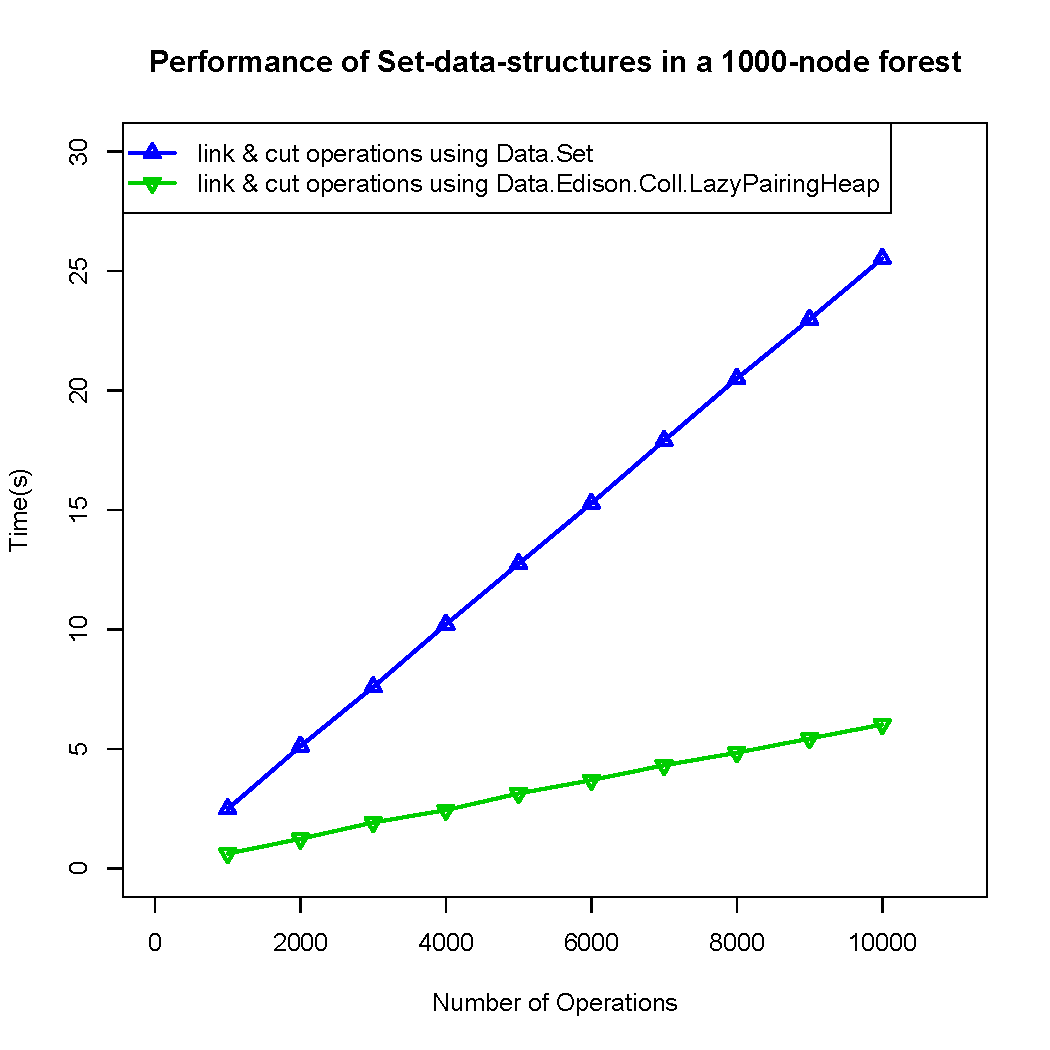
\includegraphics[scale=0.4]{./Images/plotSets} 
\end{center}
\caption{Dynamic operations through different sets structures as monoidal annotations}
\label{fig:plotSets}
\end{figure}

The above curves show that, although by a constant factor, laziness speeds up the running time in the computation of dynamic tree operations through the set-like data structures.

\tcb{Amortised over what??}
